\chapter{Design} \label{cha:design}
\section{Technology Choices} \label{sec:chapdesign:technology}
This section will discuss choices that have been made throughout the project regarding technology used and justifications for their usage.

\subsection{Rust} \label{sec:chapdesign:technology:rust}
There were a few requirements when choosing an appropriate programming language for this project:
\begin{enumerate} 
    \item Performance: There are two aspects to performance within this project. Performance considerations and optimization are vital on IOT devices themselves, due to their limited on-board processing power. On the other hand, while performance on servers is definitely important, it is significantly easier to scale server-performance, by simply adding more servers (horizontal scaling) or by improving the hardware of any individual server (vertical scaling), than it is to improve performance of an IoT device. This is especially true of an IoT device that is already deployed.
    \item Stability: Another important requirement when choosing a language is the stability of code written in the language. This does not necessarily mean that code written in any language is inherently unstable. This requirement is more of a consideration about if a language enables and encourages a programmer to write code that is memory-safe and handles errors correctly. This is important in an IoT environment, as devices are expected to run for long periods. What is the point of a security camera if it's software crashes every couple days, due to an obscure memory out of bounds error? 
    \item Security: While no language is inherently "hack-proof" or secure, there are ways a language can encourage behaviors that can lead to better outcomes in security. A blog-post by the "Microsoft Security Response Centre" states that 70\% of all vulnerabilities assigned a CVE (Common Vulnerabilities and Exposures) each year are due to memory corruption errors \cite{ProactiveApproachToSecureCode}. In the post the languages "C" and "C++" are specifically referred to as being part of this problem. As mentioned in subsection ~\ref{sec:chap2:security}, security is of particular importance in smart home systems, so ensuring a method or language that enables secure code is chosen is of particular importance. 
    \item Ease of Use and Comfort: While not particularly important in the final product, having a language that is easy to develop in can make the developer experience easier and can lead to faster iteration on ideas, perhaps leading to a better final result. That being said, developer familiarity with a language can more than make up this difference. A seasoned C++ developer will be able to iterate faster and produce a better product in C++, than if they are using an "easy" language, that they are not as familiar with.
\end{enumerate}\todo{not sure I like the list style here}
After some deliberation, the language that was chosen for this project was Rust. While C/C++'s performance rivals and often surpasses Rust, the difference is often quite marginal \cite{PerformanceEvalOnMicrocontroller}, due to all three being compiled to machine code. What makes Rust different, is its headline feature, known as the "borrow checker". While the details of the borrow checker are out of scope of this paper, it can ensure that at compile-time, the code is memory safe. While there are ways to circumvent this (using the "unsafe" keyword), this has to be explicitly done. Due to the code being guaranteed memory safe at compile time, outside the aforementioned unsafe blocks, Rust code is known for its ability to run long-term without running into crashes. Additionally, Rust code is a popular choice for embedded devices, due to being able to compile without a standard library (this has to be enabled), giving it flexibility in a project such as this.

I have decided to use Rust for both the Server and Clients. While Rust might be a somewhat obvious choice for IoT clients, it is less so for servers. Due to the "borrow checker", while Rust might be safe, it is often said to be harder to write than traditional languages. This makes it more questionable as the primary language for the server, due to it being a less constrained platform (view performance section above). While servers are theoretically almost infinitely horizontally scalable, in practice this is often not the case, especially in a smart-home's case, as they have to fit in someone's home and generally should be affordable. Therefore, ensuring that the server can run on as many devices as possible, be it a Raspberry-Pi, or a modern desktop, is an important goal to strive for. The "difficulty" aspect of Rust can be largely counteracted by personal familiarity with the language. Additionally, having a stable server is very important, especially since all IoT devices will need to frequently communicate with this server, an aspect which Rust excels at. Rust also has a thriving community of libraries (known as crates), which using the language gives access to. For these reasons I have chosen Rust as the primary programming language of the Server and Client parts of this project.

Note that the words crate and library will be used interchangeably throughout this report, due to them being very similar concepts, but library being more familiar to non-rust users. 

\subsection{gRPC} \label{sec:chapdesign:technology:grpc}
gRPC is an RPC implementation released by Google in 2015. It uses Protocol Buffers (protobufs) as an interface definition language (IDL), to define services on servers, that clients can then call, such as any RPC library. The server runs a gRPC server and the client runs the gRPC client \cite{grpcHomepage}. Protobufs are compiled to many different languages, with many different libraries available for these languages, that automate much of the process. In a performance comparison between REST, gRPC, websockets, GraphQL, gRPC came out ahead in many different metrics \cite{reviewOfInternetProtocols}. These include: 
\begin{itemize}
    \item inserting one value into a database
    \item fetching one value from a database 
    \item fetching one hundred elements  
\end{itemize}
in both native and containerized tests. In fact, gRPC was the most performant internet communication protocol in all metrics apart from memory usage.

Due to its performance and cross-language support I have chosen gRPC as the internet communication protocol for this project. The specific library used for this project is known as "Tonic". Tonic is a Rust gRPC crate that includes both a gRPC server and client. It also utilizes "prost" to compile protobuf files into Rust code, without having to interface the protobuf compiler itself. All protobuf files are compiled as a compilation step of the server and client, eliminating the need for external build scripts (this is only partially true, view Sub Section~\ref{sec:chapdesign:server:protoBufs}).

\subsection{Typescript \& VueJS} \label{sec:chapdesign:technology:ts}
While a Command Line Interface (CLI) frontend, written in Rust, will be made available, the main focus will be on the Graphical User Interface (GUI). To ensure that it can run on a variety of systems and is relatively easy to create, it will be web based, using Javascript at runtime. However, it will be written in Typescript. Typescript is a superset of Javascript, that compiles to Javascript and leaves no trace of types behind. Typescript provides a robust type-system, including, but not limited to \cite{understandingTypescript}:
\begin{itemize}
    \item Structural type equivalence, instead of Javascript's by-name type equivalence
    \item Types and concepts for object-based programming
    \item Type operators
\end{itemize}
All of these, while not guaranteeing that the program will be type-safe at runtime, help a developer design more robust and long term solutions generally associated with statically typed languages.

In conjunction with Typescript a web-development framework will be used. Web frameworks are libraries for Javascript that allow easier development of websites and web apps, often incorporating HTML (HyperText Markup Language) and CSS (Cascading Style Sheets) code into Javascript code. They also provide reactivity, meaning that if a variable changes in the code, that change can easily be reflected on the site. This can be done in most frameworks by simply using the variable in the HTML code, something that standard HTML does not support (methods of doing this differs between frameworks).

Most of the choice between different web-frameworks comes down to personal preference and familiarity with a framework. That being said there can be performance differences between different frameworks, that could make a difference on some systems. While there is a lack of formal experiments on framework performance, an informal experiment \cite{performanceComparisonJS} showed that while there is a performance difference between different frameworks, it should not be the primary decision maker. When the difference when creating 1000 rows between vanilla JavaScript and VueJS is 32 milliseconds, the disparity will not be noticeable to the end user. For this reason, and personal familiarity with the framework, I have decided to use VueJS as the frontend development framework for this project.

\section{System Architecture} \label{sec:chapdesign:architecture}

The overall system architecture can be seen in figure~\ref{fig:system_architecture}.
\begin{figure}[h]
\caption{System Architecture}
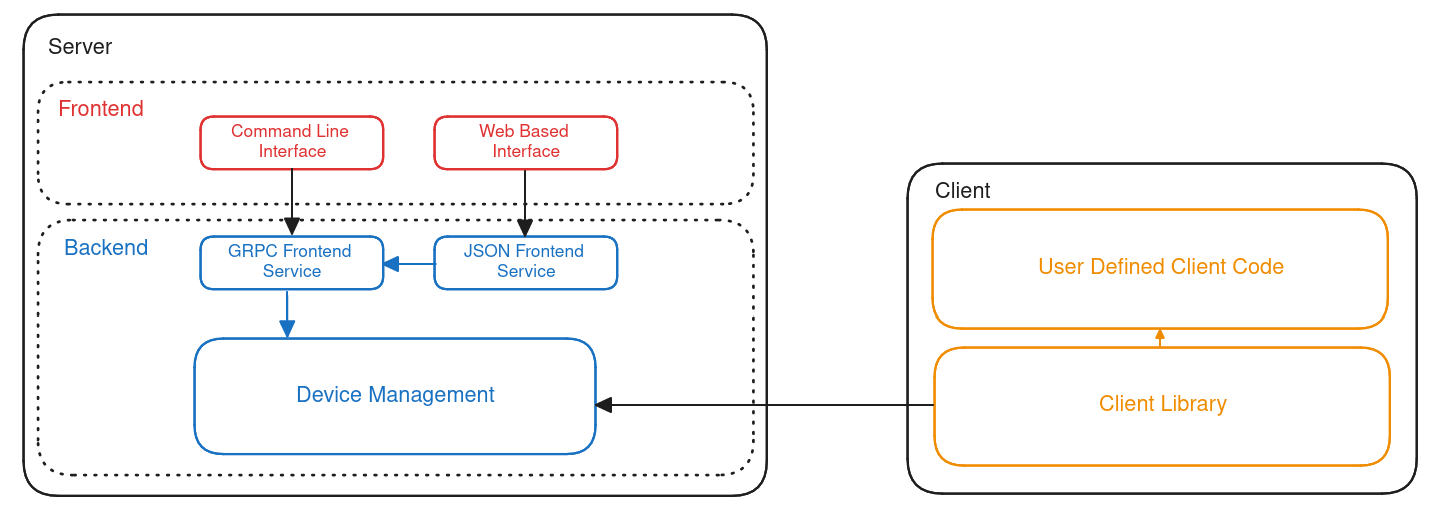
\includegraphics[width=\textwidth]{system_architecture.png}
\label{fig:system_architecture}
\end{figure}
This system architecture consists of two main components, the server and the client. Here the server represents the main controller of the system. The client is any device connected to the system (there most likely will be multiple). One peculiarity, is the fact that the frontend is contained by the server part of the system. This is because, in the current design, by default the frontend will be run on the same machine as the backend, with frontend API endpoints (located in the frontend services) being open on the localhost loop back address. This can however be easily changed by a user, by simply changing the address the frontend API endpoints are hosted on.

The arrows in the architectural diagram represent the direction of contact. For example, a client can contact the backend and the backend may respond, however the backend cannot contact a device, it can only reply to a request. The only deviation from this rule is within the client. At startup, the user will supply the client library with callback functions, which the library can call. This means that the user defined code must be able to contact the client library during setup. However, once the client library has finished setup and has created contact with the backend, the user defined code can no longer interact directly with the client library. The library will then simply call any code supplied to it during setup, without having any direct contact with user defined code.

\section{Security} \label{sec:chapdesign:security}
As previously discussed, security is an important concern within a smart-home environment. The user of the system is putting trust into the system to behave as it is meant to, while keeping their personal data safe from outside intruders. That is why special care will be put into the security aspects of the system. This will come in a two pronged approach using certificates and signatures. 
\subsection{Certificates}
\todo{think about including timestamp in certificate}
A certificate is a tool for verifying that a client is who they say they are. It is generated by the server and can be verified by the server. This is useful, for example, if the client goes offline and at a later time wants to re-aunthenticate with the server. They can send the certificate provided to them earlier and the server can verify it. The certificate scheme that will be implemented is based on \cite{disSysConceptsDesign}.

Figure~\ref{fig:certificate_exchange} shows the certificate exchange protocol that will be used, where cK is the client key pair and sK is the server key pair. K(pub) represents the public key part of the key pair.
\begin{figure}[h]
\caption{Certificate Exchange}
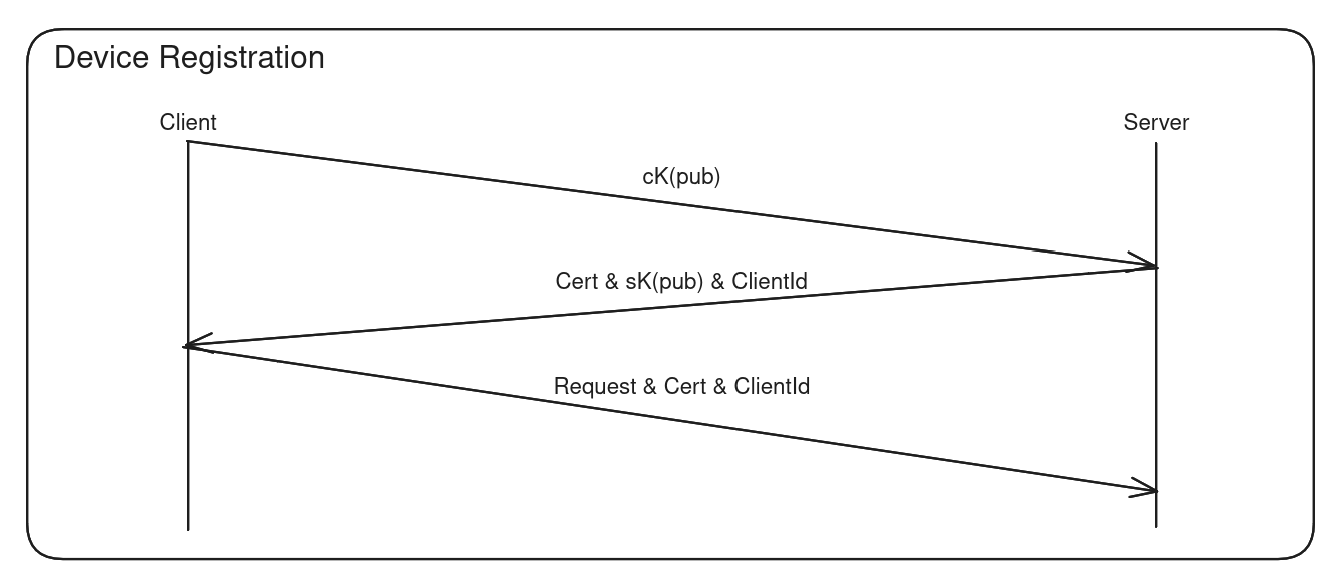
\includegraphics[width=\textwidth]{certificate_exchange.png}
\label{fig:certificate_exchange}
\end{figure}

At startup the server and client will both generate an asymmetric key pair using the Rivest, Shamir, Adleman (RSA) public key system. Then, during registration, the client will send the server their public key. The server then creates csr where \(csr = cK(pub) + ClientId\). Csr is then hashed using SHA256 hashing to create the certificate: \(certificate = H_x(csr)\). This certificate is then sent back to the client, along with the server public key and their client identifier (which is a UUID randomly generated by the server). Now, if the client goes offline and wants to re-register, instead of having to repeat the registration process again, they can simply include their certificate instead and be verified by the server. Verification is quite simple. The client simply re-generates csr using the client's public key and client-id, then re-hashes them. If the new hash is the same as the certificate, then the client is verified.

\subsection{Signatures}
Signatures allow both the server and client to verify that the messages they are receiving are not forged and sent by a third party. The signatures will use the key-pairs generated and exchanged during registration (view certificate exchange), to sign every message with a hash, that can be independently verified by the other party. The message sender will use their private key to sign their message and the receiver will use the public key send during registration to verify the message. This signature scheme is based on concepts described within \cite{disSysConceptsDesign} and \cite{disSysPrinciples}.

Every signature will consist of three important parts:
\begin{enumerate}
    \item Unix Timestamp - This will be used to prevent replay attacks. Every message will include the Unix timestamp of when it was sent and this information will be included in the signature. The receiver can then check the age of the message and discard it if it is beyond a certain threshold.
    \item Message Contents - This is used to ensure that the contents of the message stay the same between sender and receiver. Because hashing the entire contents of a message might be costly, some subset of the contents must be chosen. This will depend on the message type.
    \item Certificate - The certificate is included in the hash, however not in the message. This is an extra layer of security, as both server and client have an independent version of the certificate, meaning that an attacker would also need to obtain this certificate somehow, along with the private key of the sender.
\end{enumerate}

Every message will include a signature, which must first be verified by the receiver before the information within the message is processed. This is help ensure that data can not be tampered with between sender and receiver.


\section{Web Frontend} \label{sec:chapdesign:frontend}
Figure~\ref{fig:home_screen_mockup} shows a mockup what the home-screen of the web frontend should look like. The main focus should be on the devices, which will be represented by boxes on the home screen. The device's available capabilities will be shown as buttons or sliders, configurable from the device itself. As the focus of this project is mainly on the system and the API of the device server will be available, custom web frontends should be easy to make, for a more customizable experience. Due to the whole project being open-source, this frontend can be built upon by other users, or companies, interested in customizing it.

\begin{figure}[h]
\caption{Home Screen Mockup}
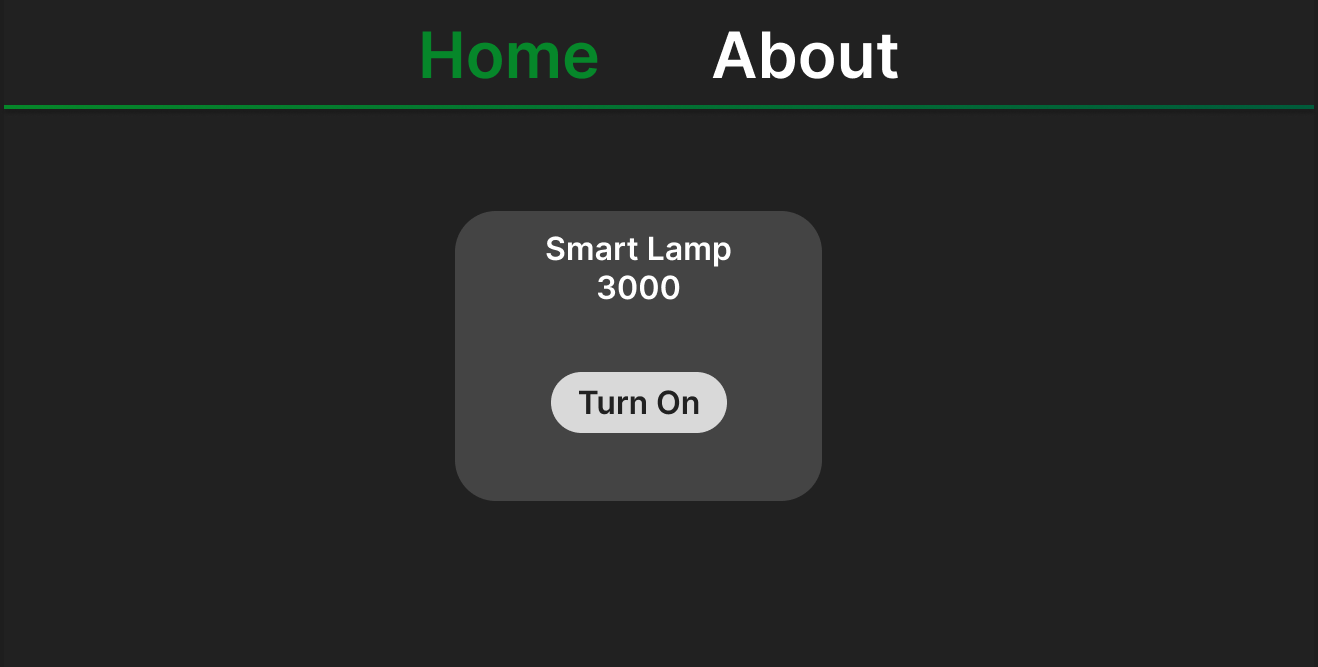
\includegraphics[width=\textwidth]{homescreen_design.png}
\label{fig:home_screen_mockup}
\end{figure}

